En la figura \ref{fig:AoN}, puede observarse el diagrama de \textit{Activity on Node} con el respectivo camino crítico. 
La unidad de tiempo \textbf{T}  se encuentra expresada en horas.

\vspace{5mm} %5mm vertical space

\begin{figure}[htpb]
	\centering
	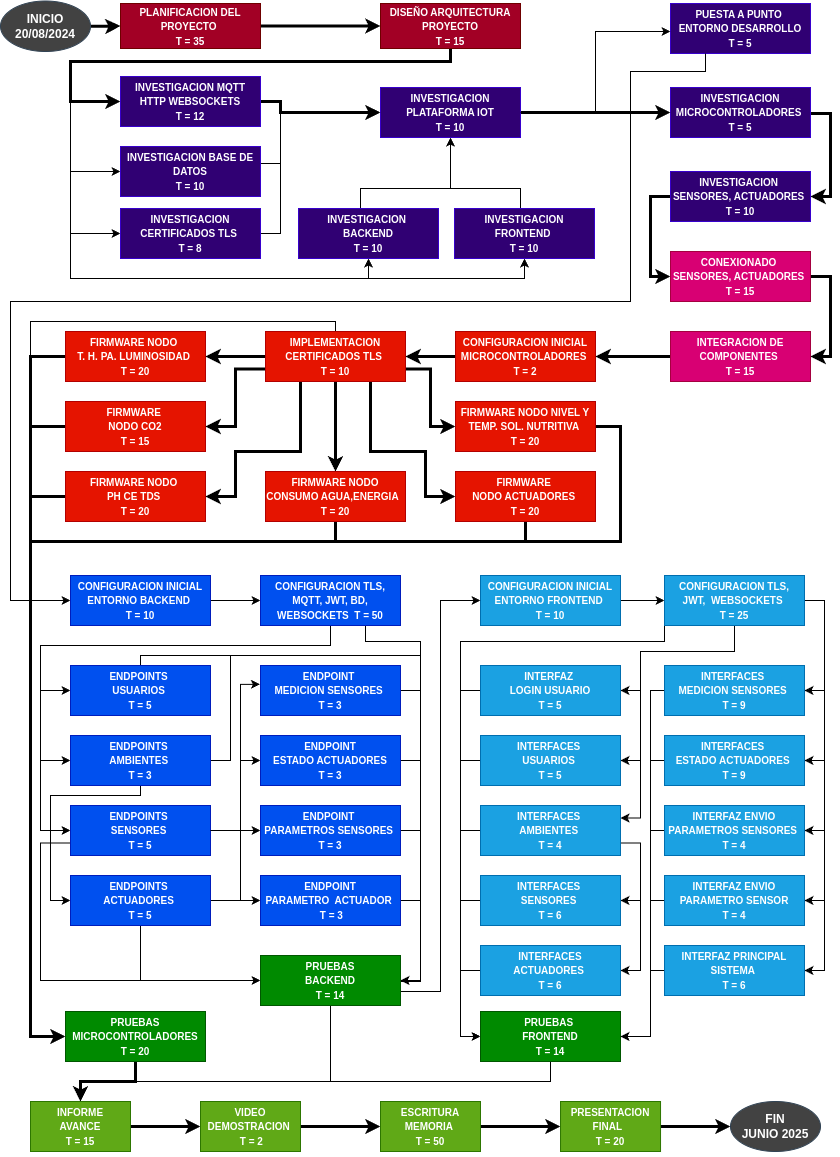
\includegraphics[width=.84\linewidth]{./Figuras/AoN.png}
	\caption{Diagrama de \textit{Activity on Node}.}
	\label{fig:AoN}
\end{figure}

\pagebreak
En la siguiente figura pueden observarse las correspondientes referencias del diagrama de \textit{Activity on Node}.

\begin{figure}[htpb]
	\begin{flushleft}
	\end{flushleft}
	\centering
	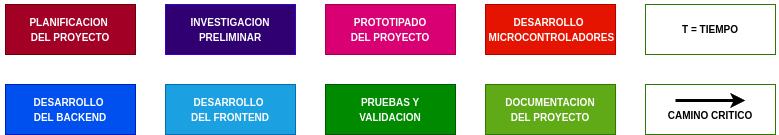
\includegraphics[width=.99\textwidth]{./Figuras/AoN_Detalle.png}
	\caption{Referencias del diagrama \textit{Activity on Node}.}
	\label{fig:AoN_Detail}
\end{figure}
